%%% Preamble
\documentclass[12pt,a4paper]{article}
\usepackage{appendix}
\usepackage{amsmath}
\usepackage{amssymb}
\makeatletter
\newcommand{\rmnum}[1]{\romannumeral #1}
\newcommand{\Rmnum}[1]{\expandafter\@slowromancap\romannumeral #1@}
\makeatother

% packages
\usepackage[T1]{fontenc}
\usepackage{fourier}
\usepackage{geometry}
\usepackage[english]{babel}															% English language/hyphenation
\usepackage[protrusion=true,expansion=true]{microtype}	
\usepackage{amsmath,amsfonts,amsthm} % Math packages
\usepackage[pdftex]{graphicx}	
\usepackage{url}
\usepackage{float}
\usepackage{indentfirst}

\geometry{left=1.0in,right=1.0in,top=1.0in,bottom=1.0in}

\usepackage{pdfpages}

%%% Begin document
\begin{document}

\begin{figure}[H] %指定浮动体排版位置 h-here t-top b-bottom p-page
	\centering %居中排版,只在环境里有这个命令,故只对环境生效
	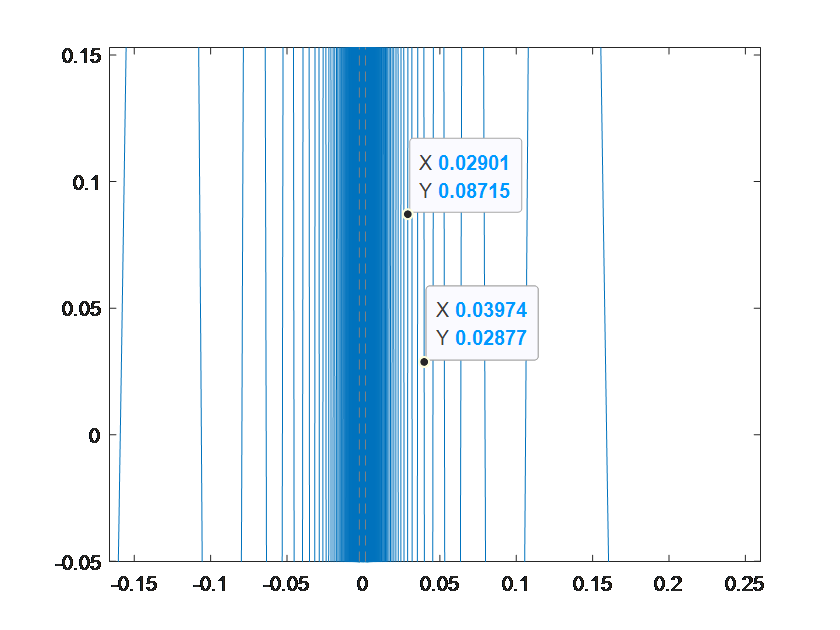
\includegraphics[height=8cm]{./word.png}
	\caption{Word} %在图下方
\end{figure}

\begin{figure}[H] %指定浮动体排版位置 h-here t-top b-bottom p-page
	\centering %居中排版,只在环境里有这个命令,故只对环境生效
	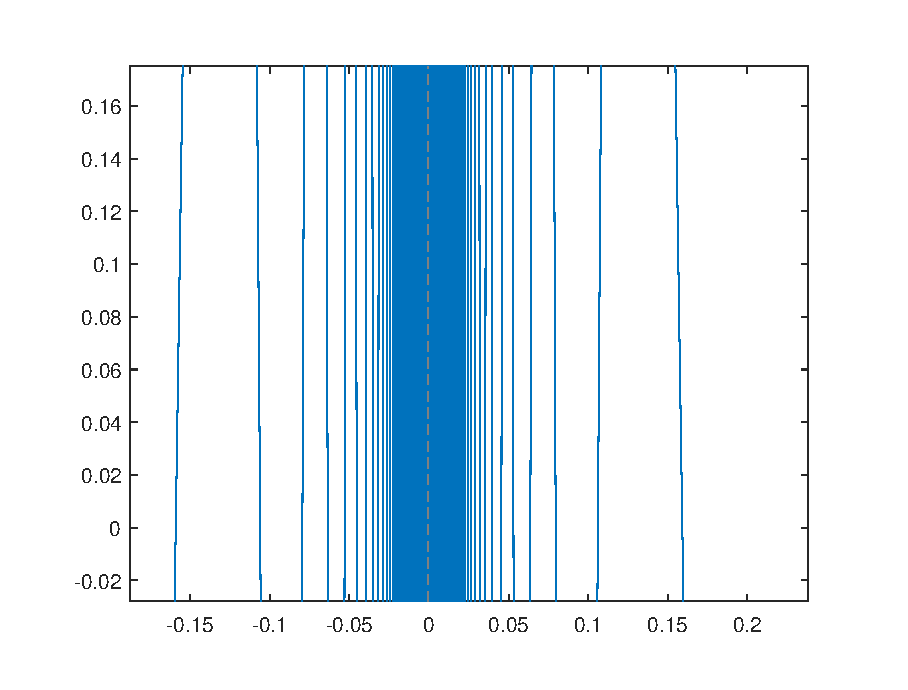
\includegraphics[height=8cm]{./eps.eps}
	\caption{EPS} %在图下方
\end{figure}

\begin{figure}[H] %指定浮动体排版位置 h-here t-top b-bottom p-page
	\centering %居中排版,只在环境里有这个命令,故只对环境生效
	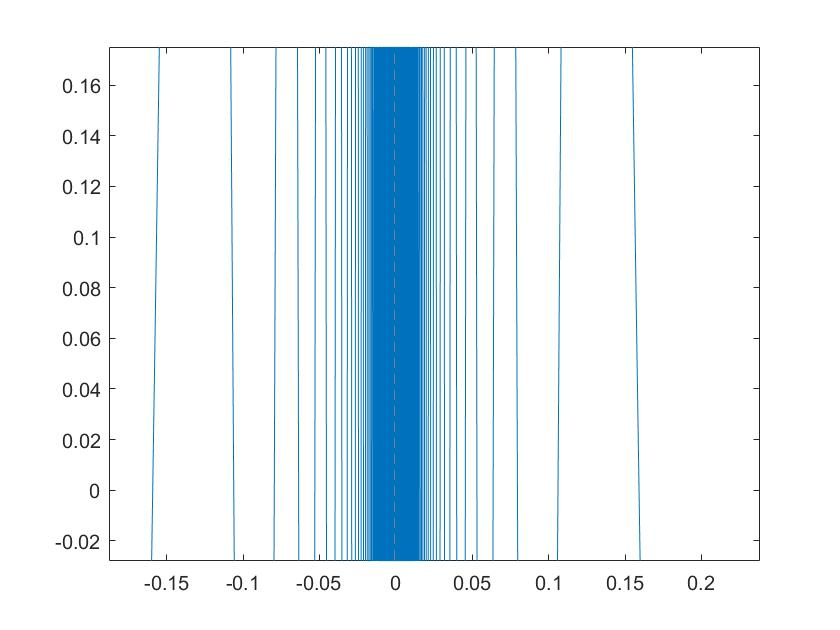
\includegraphics[height=8cm]{./jpg.jpg}
	\caption{Matlab} %在图下方
\end{figure}

\end{document}